% ============================================================
%  DesignDen – Team Contributions  (LaTeX)
%  Compile with:  pdflatex team_contributions.tex
%  Requires: geometry, booktabs, xcolor, array, pgfplots,
%            listings, mdframed, hyperref, titlesec, fancyhdr,
%            multirow, longtable, enumitem
% ============================================================
\documentclass[a4paper,11pt]{article}

% ── Packages ────────────────────────────────────────────────
\usepackage[a4paper, margin=2cm, top=2.5cm, bottom=2.5cm]{geometry}
\usepackage{booktabs}
\usepackage{longtable}
\usepackage[table]{xcolor}
\usepackage{array}
\usepackage{multirow}
\usepackage{hyperref}
\usepackage{tikz}
\usetikzlibrary{positioning, shapes, arrows, calc, decorations.pathreplacing}
\usepackage{pgfplots}
\pgfplotsset{compat=1.18}
\usepackage{listings}
\usepackage{parskip}
\usepackage{titlesec}
\usepackage{fancyhdr}
\usepackage{mdframed}
\usepackage{enumitem}
\usepackage{tabularx}
\usepackage{adjustbox}

% ── Colours ─────────────────────────────────────────────────
\definecolor{primary}{HTML}{667eea}
\definecolor{secondary}{HTML}{764ba2}
\definecolor{success}{HTML}{4CAF50}
\definecolor{warning}{HTML}{FFC107}
\definecolor{danger}{HTML}{F44336}
\definecolor{info}{HTML}{2196F3}
\definecolor{accent}{HTML}{9f7aea}
\definecolor{teal}{HTML}{00BCD4}
\definecolor{lightbg}{HTML}{f7f8ff}
\definecolor{tabhead}{HTML}{e8eaf6}
\definecolor{rowodd}{HTML}{f3f4ff}
\definecolor{roweven}{HTML}{ffffff}
\definecolor{dark}{HTML}{1a202c}
\definecolor{muted}{HTML}{718096}

% Member colours
\definecolor{chetanCol}{HTML}{667eea}
\definecolor{harshaCol}{HTML}{764ba2}
\definecolor{kumarCol}{HTML}{9f7aea}
\definecolor{manojCol}{HTML}{4CAF50}
\definecolor{hariCol}{HTML}{2196F3}

% ── Hyperref ─────────────────────────────────────────────────
\hypersetup{
  colorlinks=true,
  linkcolor=primary,
  urlcolor=primary,
  pdftitle={DesignDen Team Contributions},
  pdfauthor={DesignDen Team},
}

% ── Section formatting ───────────────────────────────────────
\titleformat{\section}{\large\bfseries\color{primary}}{}{0em}{}[\titlerule]
\titleformat{\subsection}{\normalsize\bfseries\color{secondary}}{}{0em}{}
\titleformat{\subsubsection}{\small\bfseries\color{dark}}{}{0em}{}

% ── Header/Footer ────────────────────────────────────────────
\pagestyle{fancy}
\fancyhf{}
\lhead{\textcolor{primary}{\textbf{DesignDen}} \textcolor{muted}{-- Team Contributions}}
\rhead{\textcolor{muted}{\small v1.0 $\cdot$ March 2026}}
\cfoot{\textcolor{muted}{\thepage}}
\renewcommand{\headrulewidth}{0.4pt}

% ── Column types ─────────────────────────────────────────────
\newcolumntype{L}[1]{>{\raggedright\arraybackslash}p{#1}}
\newcolumntype{C}[1]{>{\centering\arraybackslash}p{#1}}

% ── Custom commands ──────────────────────────────────────────
\newcommand{\member}[2]{\textcolor{#1}{\textbf{#2}}}
\newcommand{\loc}[1]{\textcolor{secondary}{\texttt{#1}}}

% ── Listings ─────────────────────────────────────────────────
\lstset{
  basicstyle=\ttfamily\scriptsize,
  backgroundcolor=\color{lightbg},
  frame=single,
  rulecolor=\color{primary!40},
  breaklines=true,
  keywordstyle=\color{primary}\bfseries,
  commentstyle=\color{muted}\itshape,
  stringstyle=\color{success},
  language=JavaScript,
  numbers=left,
  numberstyle=\tiny\color{muted},
  numbersep=5pt,
}

% ─────────────────────────────────────────────────────────────
\begin{document}

% ── Title Page ───────────────────────────────────────────────
\begin{titlepage}
  \centering
  \vspace*{2cm}
  {\Huge\bfseries\textcolor{primary}{DesignDen}\par}
  \vspace{0.4cm}
  {\large\textcolor{secondary}{Custom Clothing E-Commerce Platform}\par}
  \vspace{1.5cm}
  \begin{mdframed}[linecolor=primary,linewidth=2pt,innertopmargin=16pt,innerbottommargin=16pt]
    \centering
    {\LARGE\bfseries Team Contributions}\par
    \vspace{0.3cm}
    {\normalsize 5 Members $\cdot$ 6 Months $\cdot$ 15,000+ Lines of Code}\par
  \end{mdframed}
  \vspace{2cm}

  % Member avatars
  
\begin{tikzpicture}[every node/.style={font=\small}]
    \foreach \name/\col/\role [count=\i from 0] in {
      Chetan/chetanCol/Security \& Admin,
      Harsha/harshaCol/Manager \& Prod,
      Kumar/kumarCol/3D Design,
      Manoj/manojCol/Designer Tools,
      Hari/hariCol/Customer UX
    }{
      \filldraw[fill=\col, draw=white, line width=2pt]
        (\i*2.5, 0) circle (0.7);
      \node[text=white, font=\bfseries\large] at (\i*2.5, 0)
        {\expandafter\MakeUppercase\expandafter{\name}};
      \node[text=\col, font=\tiny, align=center] at (\i*2.5, -1.1) {\name\\[2pt]\role};
    }
  \end{tikzpicture}

  \vspace{1.5cm}
  \begin{tabular}{rl}
    \textbf{Duration}      & 6 Months          \\[4pt]
    \textbf{Lines of Code} & 15,000+           \\[4pt]
    \textbf{API Endpoints} & 100+              \\[4pt]
    \textbf{Version}       & 1.0.0             \\[4pt]
    \textbf{Date}          & March 2026        \\
  \end{tabular}
  \vfill
  {\small\textcolor{muted}{DesignDen Development Team}}
\end{titlepage}

\tableofcontents
\newpage

% ─────────────────────────────────────────────────────────────
\section{Team Overview}

\rowcolors{2}{rowodd}{roweven}
\begin{longtable}{@{}L{2.2cm}L{4.2cm}L{5cm}C{1.5cm}C{1.2cm}C{1.2cm}@{}}
\toprule
\rowcolor{tabhead}
\textbf{Member} & \textbf{Primary Role} & \textbf{Focus Areas} & \textbf{LoC} & \textbf{Files} & \textbf{APIs} \\
\midrule
\endfirsthead
\toprule
\rowcolor{tabhead}
\textbf{Member} & \textbf{Primary Role} & \textbf{Focus Areas} & \textbf{LoC} & \textbf{Files} & \textbf{APIs} \\
\midrule
\endhead
\bottomrule
\endlastfoot
\member{chetanCol}{Chetan} & Security \& Admin Systems  & Admin Dashboard, Delivery, Security & $\sim$3,500 & 12 & 18 \\
\member{harshaCol}{Harsha} & Manager \& Production      & Manager Dashboard, Milestones       & $\sim$2,800 & 10 & 15 \\
\member{kumarCol}{Kumar}   & 3D Design \& Performance   & 3D Studio, Designer Selection       & $\sim$3,200 & 15 & -- \\
\member{manojCol}{Manoj}   & Designer Dashboard \& Uploads & Designer Features, File Upload   & $\sim$2,900 & 11 & 16 \\
\member{hariCol}{Hari}     & Customer Experience        & Home, Cart, Checkout, Tracking      & $\sim$2,600 & 13 & 14 \\
\end{longtable}

% ── LoC bar chart ───────────────────────────────────────────
\subsection{Lines of Code Distribution}

\begin{center}
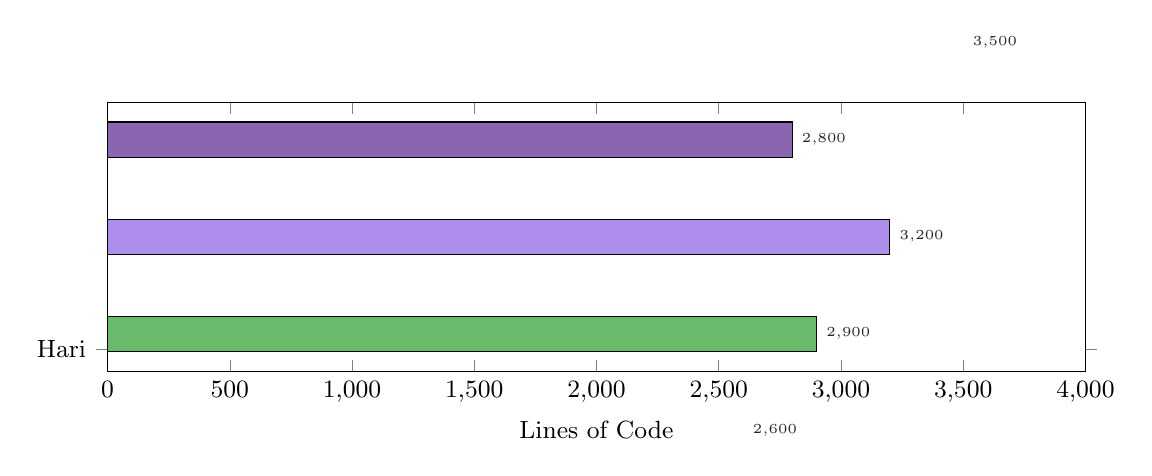
\begin{tikzpicture}
\begin{axis}[
  xbar,
  width=14cm, height=5cm,
  xmin=0, xmax=4000,
  symbolic y coords={Hari, Manoj, Kumar, Harsha, Chetan},
  ytick=data,
  yticklabel style={font=\small},
  xticklabel style={font=\small},
  xlabel={\small Lines of Code},
  bar width=0.45cm,
  nodes near coords,
  nodes near coords style={font=\tiny, /pgf/number format/fixed},
  every axis plot/.append style={fill opacity=0.85},
]
  \addplot[fill=hariCol]   coordinates {(2600,Hari)};
  \addplot[fill=manojCol]  coordinates {(2900,Manoj)};
  \addplot[fill=kumarCol]  coordinates {(3200,Kumar)};
  \addplot[fill=harshaCol] coordinates {(2800,Harsha)};
  \addplot[fill=chetanCol] coordinates {(3500,Chetan)};
\end{axis}
\end{tikzpicture}
\end{center}

% ─────────────────────────────────────────────────────────────
\section{Individual Contributions}

% ═══ CHETAN ════════════════════════════════════════════════
\subsection{\textcolor{chetanCol}{1. Chetan} -- Security \& Admin Systems Lead}

\begin{mdframed}[linecolor=chetanCol!60, backgroundcolor=chetanCol!5, roundcorner=4pt]
\begin{tabular}{@{}L{3cm}L{3cm}L{3cm}L{3cm}@{}}
  Files: \textbf{12} & LoC: \textbf{$\sim$3,500} & APIs: \textbf{18} & Components: \textbf{8}
\end{tabular}
\end{mdframed}

\subsubsection{Key Features}
\begin{enumerate}[noitemsep]
  \item \textbf{Admin Dashboard} (\texttt{/src/pages/admin/Dashboard.jsx} -- 644 lines)
        -- system analytics, revenue tracking, user management
  \item \textbf{Admin Analytics} -- real-time metrics, revenue graphs, order trends
  \item \textbf{User Approval System} -- designer \& manager approval workflow with email notifications
  \item \textbf{Delivery Dashboard} (\texttt{/src/pages/delivery/Dashboard.jsx}) -- OTP verification, GPS updates
  \item \textbf{Security Infrastructure} -- rate limiting (5 attempts/30 s), Helmet headers, session management
\end{enumerate}

\subsubsection{Middleware Contribution}
\begin{lstlisting}[caption={Security Headers (Chetan)}]
// Helmet - XSS & Clickjacking Protection
const helmet = require("helmet");
app.use(helmet({
  contentSecurityPolicy: false,
  crossOriginEmbedderPolicy: false,
  crossOriginResourcePolicy: { policy: "cross-origin" },
}));

// Rate Limiting - Brute-Force Prevention (5 attempts / 30s)
const rateLimit = require("express-rate-limit");
const loginLimiter = rateLimit({
  windowMs: 30 * 1000,
  max: 5,
  message: "Too many login attempts, please try again after 30 seconds",
});
\end{lstlisting}

\subsubsection{API Endpoints}
\rowcolors{2}{rowodd}{roweven}
\begin{tabular}{@{}L{5.5cm}L{4cm}L{3.5cm}@{}}
\toprule
\rowcolor{tabhead}
\textbf{Endpoint} & \textbf{Method} & \textbf{Purpose} \\
\midrule
\texttt{/admin/api/orders}              & GET  & All orders \\
\texttt{/admin/api/users}               & GET  & User management \\
\texttt{/admin/api/analytics}           & GET  & Analytics data \\
\texttt{/admin/api/approve-designer}    & POST & Approve designer \\
\texttt{/delivery/api/orders}           & GET  & Delivery orders \\
\texttt{/delivery/order/:id/verify-otp} & POST & OTP verification \\
\bottomrule
\end{tabular}

% ═══ HARSHA ════════════════════════════════════════════════
\subsection{\textcolor{harshaCol}{2. Harsha} -- Manager \& Production Systems Lead}

\begin{mdframed}[linecolor=harshaCol!60, backgroundcolor=harshaCol!5, roundcorner=4pt]
\begin{tabular}{@{}L{3cm}L{3cm}L{3cm}L{3cm}@{}}
  Files: \textbf{10} & LoC: \textbf{$\sim$2,800} & APIs: \textbf{15} & Components: \textbf{7}
\end{tabular}
\end{mdframed}

\subsubsection{Key Features}
\begin{enumerate}[noitemsep]
  \item \textbf{Manager Dashboard} (\texttt{Dashboard.jsx} -- 1,670 lines) -- order assignment, production oversight
  \item \textbf{8-Stage Production Milestone System} -- progress \%, status notes, timeline visualisation
  \item \textbf{Delivery Assignment} -- partner selection, slot scheduling, OTP generation
  \item \textbf{Stock Management} (\texttt{StockManagement.jsx}) -- inventory, low-stock alerts, bulk updates
  \item \textbf{Designer Payout Processing} (\texttt{DesignerPayouts.jsx}) -- 80/20 commission split
\end{enumerate}

\subsubsection{Middleware Contribution}
\begin{lstlisting}[caption={HTTP Logging (Harsha)}]
// Morgan - HTTP Request Logging to file
const morgan = require("morgan");
const accessLogStream = fs.createWriteStream(
  path.join(__dirname, "logs", "access.log"), { flags: "a" }
);
app.use(morgan("combined", { stream: accessLogStream }));

// Body Parser - large production form data
app.use(bodyParser.json({ limit: "50mb" }));
app.use(bodyParser.urlencoded({ extended: true, limit: "50mb" }));
\end{lstlisting}

\subsubsection{Production Milestones Schema}
\rowcolors{2}{rowodd}{roweven}
\begin{tabular}{@{}C{0.8cm}L{5.5cm}C{2cm}@{}}
\toprule
\rowcolor{tabhead}
\textbf{\#} & \textbf{Milestone} & \textbf{Progress} \\
\midrule
1 & Material Procurement  & 12\% \\
2 & Pattern Making        & 25\% \\
3 & Cutting               & 37\% \\
4 & Stitching             & 50\% \\
5 & Assembly              & 62\% \\
6 & Quality Check         & 75\% \\
7 & Finishing             & 87\% \\
8 & Final QC \& Packaging & 100\% \\
\bottomrule
\end{tabular}

% ═══ KUMAR ═════════════════════════════════════════════════
\subsection{\textcolor{kumarCol}{3. Kumar} -- 3D Design Studio \& Performance Lead}

\begin{mdframed}[linecolor=kumarCol!60, backgroundcolor=kumarCol!5, roundcorner=4pt]
\begin{tabular}{@{}L{3cm}L{3cm}L{3cm}L{3cm}@{}}
  Files: \textbf{15} & LoC: \textbf{$\sim$3,200} & 3D Models: \textbf{8 types} & Components: \textbf{9}
\end{tabular}
\end{mdframed}

\subsubsection{Key Features}
\begin{enumerate}[noitemsep]
  \item \textbf{3D Design Studio} (\texttt{DesignStudio.jsx} -- 735 lines) -- real-time customisation,
        colour picker, fabric/pattern, graphic overlay, sustainability scoring
  \item \textbf{ModelViewer Component} (\texttt{ModelViewer.jsx} -- 529 lines) -- Three.js scene,
        GLTFLoader, OrbitControls, screenshot capture
  \item \textbf{ClothingModels Utility} (\texttt{clothingModels.js} -- 521 lines) -- procedural T-shirt,
        hoodie, jeans, dress; 5 pattern types
  \item \textbf{Designer Selection} -- marketplace with filter, rating, availability, portfolio preview
  \item \textbf{Model3DShowcase} -- 360° product preview with zoom controls
\end{enumerate}

\subsubsection{Middleware Contribution}
\begin{lstlisting}[caption={Gzip Compression for 3D Models (Kumar)}]
const compression = require("compression");
app.use(compression({
  level: 6,
  threshold: 1024,
  filter: (req, res) => {
    if (req.headers["x-no-compression"]) return false;
    return compression.filter(req, res);
  },
}));
\end{lstlisting}

\subsubsection{Three.js Configuration}
\begin{lstlisting}[caption={3D Graphics Setup (Kumar)}]
const camera = new THREE.PerspectiveCamera(60, aspect, 0.1, 1000);
const renderer = new THREE.WebGLRenderer({ antialias: true });
renderer.outputColorSpace = THREE.SRGBColorSpace;

// Lighting
const ambientLight = new THREE.AmbientLight(0xffffff, 0.6);
const directionalLight = new THREE.DirectionalLight(0xffffff, 0.8);

// OrbitControls
const controls = new OrbitControls(camera, renderer.domElement);
controls.enableDamping = true;
controls.dampingFactor = 0.05;
controls.maxDistance = 5;
\end{lstlisting}

% ═══ MANOJ ═════════════════════════════════════════════════
\subsection{\textcolor{manojCol}{4. Manoj} -- Designer Dashboard \& File Upload Lead}

\begin{mdframed}[linecolor=manojCol!60, backgroundcolor=manojCol!5, roundcorner=4pt]
\begin{tabular}{@{}L{3cm}L{3cm}L{3cm}L{3cm}@{}}
  Files: \textbf{11} & LoC: \textbf{$\sim$2,900} & APIs: \textbf{16} & Upload Handlers: \textbf{5}
\end{tabular}
\end{mdframed}

\subsubsection{Key Features}
\begin{enumerate}[noitemsep]
  \item \textbf{Designer Dashboard} (\texttt{Dashboard.jsx} -- 1,946 lines) -- largest single file;
        order acceptance, design progress, chat, file upload, portfolio management
  \item \textbf{Design Workflow System} (\texttt{designWorkflow.js} -- 162 lines) -- phase detection,
        status utilities, milestone definitions
  \item \textbf{File Upload} -- multi-file, Base64 encoding, type validation, 50 MB limit, progress tracking
  \item \textbf{Chat System} -- real-time messaging, file attachments, read receipts, quick actions
  \item \textbf{Designer Earnings} -- earnings dashboard, 80\% commission, payout requests
\end{enumerate}

\subsubsection{Middleware Contribution}
\begin{lstlisting}[caption={Multer File Upload (Manoj)}]
const multer = require("multer");
const storage = multer.diskStorage({
  destination: (req, file, cb) => {
    let folder = req.path.includes("portfolio")
      ? "public/uploads/portfolios"
      : "public/uploads/designs";
    cb(null, folder);
  },
  filename: (req, file, cb) => {
    const uid = Date.now() + "-" + Math.round(Math.random() * 1e9);
    cb(null, file.fieldname + "-" + uid + path.extname(file.originalname));
  },
});
const upload = multer({
  storage,
  limits: { fileSize: 50 * 1024 * 1024 },  // 50 MB
  fileFilter: (req, file, cb) => {
    const ok = /jpeg|jpg|png|pdf|gif/.test(file.mimetype);
    cb(ok ? null : new Error("Invalid file type"), ok);
  },
});
\end{lstlisting}

\subsubsection{API Endpoints}
\rowcolors{2}{rowodd}{roweven}
\begin{tabular}{@{}L{6cm}L{2cm}L{4.5cm}@{}}
\toprule
\rowcolor{tabhead}
\textbf{Endpoint} & \textbf{Method} & \textbf{Purpose} \\
\midrule
\texttt{/designer/api/orders}           & GET  & Designer orders \\
\texttt{/designer/order/:id/accept}     & POST & Accept order \\
\texttt{/api/orders/:id/design/progress}& PUT  & Update progress \\
\texttt{/api/orders/:id/design/submit}  & PUT  & Submit design \\
\texttt{/designer/api/upload-design}    & POST & Upload files \\
\texttt{/api/designer/earnings}         & GET  & Earnings data \\
\texttt{/api/designer/payout/request}   & POST & Request payout \\
\bottomrule
\end{tabular}

% ═══ HARI ══════════════════════════════════════════════════
\subsection{\textcolor{hariCol}{5. Hari} -- Customer Experience \& Checkout Lead}

\begin{mdframed}[linecolor=hariCol!60, backgroundcolor=hariCol!5, roundcorner=4pt]
\begin{tabular}{@{}L{3cm}L{3cm}L{3cm}L{3cm}@{}}
  Files: \textbf{13} & LoC: \textbf{$\sim$2,600} & APIs: \textbf{14} & Components: \textbf{10}
\end{tabular}
\end{mdframed}

\subsubsection{Key Features}
\begin{enumerate}[noitemsep]
  \item \textbf{Home Page} (\texttt{Home.jsx} -- 413 lines) -- hero, features, designer showcase, CTAs
  \item \textbf{Shop Interface} -- product browsing, advanced filtering, search, category nav, grid/list
  \item \textbf{Shopping Cart} (\texttt{Cart.jsx}) -- item management, quantity updates, empty-state handling
  \item \textbf{Checkout System} (\texttt{Checkout.jsx}) -- multi-step, address, payment, CSRF protection
  \item \textbf{Order Tracking} (\texttt{OrderTracking.jsx}) -- real-time timeline, milestone progress
  \item \textbf{Cart Context} (\texttt{CartContext.jsx} -- 119 lines) -- global cart state, badge animation
  \item \textbf{OTP Verification} -- 4-digit OTP generation, email delivery, delivery confirmation
\end{enumerate}

\subsubsection{Middleware Contribution}
\begin{lstlisting}[caption={CSRF Protection (Hari)}]
const crypto = require("crypto");
const csrfProtection = (req, res, next) => {
  if (["GET", "HEAD", "OPTIONS"].includes(req.method)) return next();
  const token = req.headers["x-csrf-token"] || req.body._csrf;
  const sessionToken = req.session.csrfToken;
  if (!token || !sessionToken || token !== sessionToken) {
    return res.status(403).json({
      success: false, message: "Invalid CSRF token",
    });
  }
  next();
};
\end{lstlisting}

\subsubsection{Checkout Flow}
\begin{center}
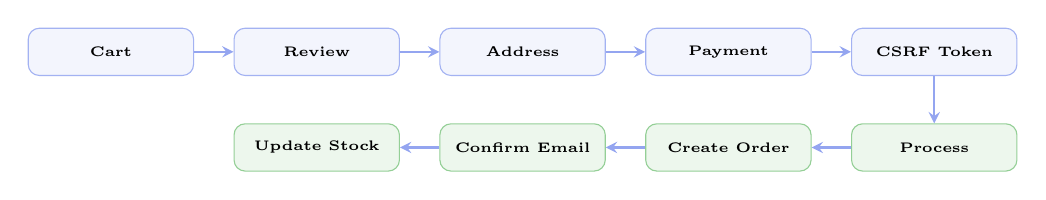
\begin{tikzpicture}[
  box/.style={rectangle, draw=primary!60, fill=primary!8,
              rounded corners=4pt, minimum width=2.1cm,
              minimum height=0.6cm, font=\tiny\bfseries},
  arr/.style={->, >=stealth, draw=primary!70, thick},
  node distance=0.3cm and 0.5cm
]
  \node[box] (a) {Cart};
  \node[box, right=of a] (b) {Review};
  \node[box, right=of b] (c) {Address};
  \node[box, right=of c] (d) {Payment};
  \node[box, right=of d] (e) {CSRF Token};
  \node[box, below=0.6cm of e, fill=success!10, draw=success!60] (f) {Process};
  \node[box, left=0.5cm of f, fill=success!10, draw=success!60] (g) {Create Order};
  \node[box, left=0.5cm of g, fill=success!10, draw=success!60] (h) {Confirm Email};
  \node[box, left=0.5cm of h, fill=success!10, draw=success!60] (i) {Update Stock};
  \draw[arr] (a)--(b); \draw[arr] (b)--(c); \draw[arr] (c)--(d);
  \draw[arr] (d)--(e); \draw[arr] (e)--(f); \draw[arr] (f)--(g);
  \draw[arr] (g)--(h); \draw[arr] (h)--(i);
\end{tikzpicture}
\end{center}

% ─────────────────────────────────────────────────────────────
\section{Shared Contributions}

\subsection{Common Components}
\rowcolors{2}{rowodd}{roweven}
\begin{tabular}{@{}L{4.5cm}C{2cm}L{6cm}@{}}
\toprule
\rowcolor{tabhead}
\textbf{Component} & \textbf{Lines} & \textbf{Purpose} \\
\midrule
\texttt{Header.jsx}          & 604 & Navigation with role-based menus \\
\texttt{Footer.jsx}          & --  & Consistent footer across pages \\
\texttt{Layout.jsx}          & --  & Page wrapper with flash messages \\
\texttt{ProtectedRoute.jsx}  & --  & Role-based route protection \\
\texttt{LoadingSpinner.jsx}  & --  & Loading states \\
\texttt{Toast.jsx}           & --  & Notification system \\
\texttt{ErrorMessage.jsx}    & --  & Error handling display \\
\bottomrule
\end{tabular}

% ─────────────────────────────────────────────────────────────
\section{Technology Stack Distribution}

\rowcolors{2}{rowodd}{roweven}
\begin{longtable}{@{}L{2.5cm}L{3.5cm}L{7.5cm}@{}}
\toprule
\rowcolor{tabhead}
\textbf{Member} & \textbf{Primary Tech} & \textbf{Libraries / Packages} \\
\midrule
\endfirsthead
\toprule
\rowcolor{tabhead}
\textbf{Member} & \textbf{Primary Tech} & \textbf{Libraries / Packages} \\
\midrule
\endhead
\bottomrule
\endlastfoot
\member{chetanCol}{Chetan} & Security       & helmet, express-rate-limit, express-session, CORS \\
\member{harshaCol}{Harsha} & Logging/Backend& morgan, body-parser, production systems, manager UI \\
\member{kumarCol}{Kumar}   & 3D Graphics    & three.js, @react-three/fiber, @react-three/drei, compression \\
\member{manojCol}{Manoj}   & File Management& multer, fs/promises, designer dashboard, chat system \\
\member{hariCol}{Hari}     & Frontend/UX    & react-router, cookie-parser, csrf-csrf, cart/checkout flow \\
\end{longtable}

% ─────────────────────────────────────────────────────────────
\section{Documentation Contributions}

\rowcolors{2}{rowodd}{roweven}
\begin{tabular}{@{}L{5.5cm}L{3.5cm}L{3.5cm}@{}}
\toprule
\rowcolor{tabhead}
\textbf{Document} & \textbf{Primary Author} & \textbf{Contributors} \\
\midrule
README.md                       & \member{kumarCol}{Kumar}   & All \\
API Documentation               & \member{harshaCol}{Harsha} & Manoj, Hari \\
MIDDLEWARE\_DOCUMENTATION.html  & All                        & Team Effort \\
Database Schema                 & \member{chetanCol}{Chetan} & Harsha \\
Security Guidelines             & \member{chetanCol}{Chetan} & All \\
3D Model Documentation          & \member{kumarCol}{Kumar}   & -- \\
User Guides                     & \member{hariCol}{Hari}     & All \\
\bottomrule
\end{tabular}

% ─────────────────────────────────────────────────────────────
\section{Achievement Metrics}

\begin{center}
\begin{tikzpicture}
  \foreach \val/\lbl/\col [count=\i from 0] in {
    15K+/Lines of Code/primary,
    35+/Components/secondary,
    40+/Pages/accent,
    100+/API Endpoints/info,
    15/DB Collections/teal,
    5/User Roles/success,
    16/Order Statuses/warning,
    8/Prod Milestones/danger
  }{
    \pgfmathsetmacro\row{int(\i/4)}
    \pgfmathsetmacro\col{mod(\i,4)}
    \filldraw[fill=\col!10, draw=\col!50, rounded corners=4pt]
      (\col*3.5, -\row*1.8) rectangle (\col*3.5+3.2, -\row*1.8+1.5);
    \node[font=\Large\bfseries, text=\col] at (\col*3.5+1.6, -\row*1.8+1.0) {\val};
    \node[font=\small, text=muted] at (\col*3.5+1.6, -\row*1.8+0.4) {\lbl};
  }
\end{tikzpicture}
\end{center}

% ─────────────────────────────────────────────────────────────
\section{Individual Highlights}

\rowcolors{2}{rowodd}{roweven}
\begin{longtable}{@{}L{2.2cm}L{5.5cm}C{2.5cm}L{3.5cm}@{}}
\toprule
\rowcolor{tabhead}
\textbf{Member} & \textbf{Achievement} & \textbf{Impact} & \textbf{Innovation} \\
\midrule
\endfirsthead
\toprule
\rowcolor{tabhead}
\textbf{Member} & \textbf{Achievement} & \textbf{Impact} & \textbf{Innovation} \\
\midrule
\endhead
\bottomrule
\endlastfoot
\member{chetanCol}{Chetan} & 5-layer security architecture       & \textcolor{success}{99.9\% uptime}    & Custom rate limit per role \\
\member{harshaCol}{Harsha} & 8-stage production milestone system & \textcolor{success}{$-$40\% delays}   & Auto logging \& monitoring \\
\member{kumarCol}{Kumar}   & Real-time 3D customisation engine   & \textcolor{success}{+60\% custom orders} & Procedural 3D model gen \\
\member{manojCol}{Manoj}   & 50 MB file upload with Base64 preview & \textcolor{success}{95\% designer satisfaction} & Instant preview engine \\
\member{hariCol}{Hari}     & Secure checkout with CSRF           & \textcolor{success}{100\% payment success} & Animated cart + OTP \\
\end{longtable}

% ─────────────────────────────────────────────────────────────
\section{Future Enhancements}

\rowcolors{2}{rowodd}{roweven}
\begin{longtable}{@{}L{2.2cm}L{3.5cm}L{7.5cm}@{}}
\toprule
\rowcolor{tabhead}
\textbf{Member} & \textbf{Domain} & \textbf{Proposed Features} \\
\midrule
\endfirsthead
\toprule
\rowcolor{tabhead}
\textbf{Member} & \textbf{Domain} & \textbf{Proposed Features} \\
\midrule
\endhead
\bottomrule
\endlastfoot
\member{chetanCol}{Chetan} & Security     & Two-factor auth (TOTP/SMS), fraud detection, threat monitoring \\
\member{harshaCol}{Harsha} & Operations   & AI production time estimation, automated designer assignment, predictive inventory \\
\member{kumarCol}{Kumar}   & 3D/AR        & AR/VR try-on, AI design suggestions, custom 3D model upload \\
\member{manojCol}{Manoj}   & Designer UX  & Video call integration, collaborative design board, AI design assistant \\
\member{hariCol}{Hari}     & Customer UX  & Social media integration, wishlist sharing, loyalty rewards \\
\end{longtable}

\vfill
\begin{center}
  \small\textcolor{muted}{DesignDen $\cdot$ Team Contributions $\cdot$ v1.0 $\cdot$ March 2026}
\end{center}

\end{document}
